\section{Existing solutions}\label{sec:existingsolutions}
In this section, some ways of achieving concurrency on an Arduino is explored. Emphasis is put on the immediate advantages and disadvantages related to each model, when considering the impact on the hobbyist users, by which is meant the new challenges, if any, introduced by the model in question.

A small sample project is implemented in each model for the sake of comparison: The builtin \gls{led} of the Arduino is set to blink - turn on and off - every half second. Concurrently, the state of a button is read and printed continously. The example will be implemented in the Arc programming language as well. The schematic for the project is seen in Figure~\ref{fig:exampleprojectschematic}.


\begin{figure}[htb!]
  \centering
  \missingfigure[figwidth=0.8\textwidth]{Insert image of Arduino schematic?}
  %\includegraphics[width=0.8\textwidth]{example-image-a}
  \caption{Example project schematic.}
  \label{fig:exampleprojectschematic}
\end{figure}


The first discussion is about the prospect of using programming libraries to achieve concurrency on an Arduino. The second discussion is about the possibility of installing an \gls{os} on the Arduino, and building on the \gls{os}-exposed concurrency abstractions.

\subsection{Concurrency through Arduino libraries}\label{subsec:arduinolibraries}
In this section, the \textit{Protothreads} and \textit{Eventually} libraries are explored and compared. Of particular concern is the quality of the documentation, the model of concurrency, and the overhead of usage on the Arduino.

\subsubsection{Protothreads}
Protothreads is a library for the C language, which has been implemented as a library for Arduino~\cite{Artin2020}. It is based on Adam Dunkels protothreads~\cite{AdamDunkelProtothreads}.


\begin{listing}[htb!]
  \centering
  \begin{minted}[label=Protothreads example]{arduino}
    #include "protothreads.h"
    #define BUTTON_PIN 12
    int buttonState = 0;  // variable for reading the pushbutton status
    pt ptBlink, ptButton;
    int blinkThread(struct pt *pt) {
      PT_BEGIN(pt);
      for (;;) {
        digitalWrite(LED_BUILTIN, HIGH); // turn the LED on (HIGH is the voltage level)
        PT_SLEEP(pt, 1000);
        digitalWrite(LED_BUILTIN, LOW); // turn the LED off by making the voltage LOW
        PT_SLEEP(pt, 1000);
      }
      PT_END(pt);
    }
    int buttonThread(struct pt *pt) {
      PT_BEGIN(pt);
      for (;;) {
        buttonState = digitalRead(BUTTON_PIN);
        Serial.println(buttonState);
        PT_YIELD(pt);
      }
      PT_END(pt);
    }
    void setup() {
      Serial.begin(9600);
      PT_INIT(&ptBlink);
      PT_INIT(&ptButton);

      pinMode(buttonPin, INPUT);
    }
    void loop() {
      PT_SCHEDULE(blinkThread(&ptBlink));
      PT_SCHEDULE(buttonThread(&ptButton));
    }
  \end{minted}
  \caption{Protothreads implementation of the sample project.}
  \label{lst:protothreadsexample}
\end{listing}


\blockcquote{Artin2020, AdamDunkelProtothreads}{Protothreads provides a blocking context on top of an event-driven system, without the overhead of per-thread stacks. The purpose of protothreads is to implement sequential flow of control without complex state machines or full multi-threading.}

The pitch for Protothreads is promising, and directly addresses the concern about overhead. However it does not describe the model of concurrency in great detail. Fortunately the documentation is excellent on both the Arduino specific implementation~\cite{Artin2020} as well as the general Protothreads specification~\cite{AdamDunkelProtothreads}.


\begin{table}[htb!]
  \centering
  \begin{tabular}{lll>{\bfseries}l}
    \toprule
    Features             & Events & Threads & Protothreads \\ \midrule
    Control structures   & no     & yes     & yes          \\
    Debug stack retained & no     & yes     & yes          \\
    Implicit locking     & yes    & no      & yes          \\
    Preemption           & no     & yes     & no           \\
    Automatic variables  & no     & yes     & no
  \end{tabular}
  \caption{Qualitative comparison between events, threads and protothreads~\cite{dunkels05using}.}
  \label{tab:protothreadscomparison}
\end{table}


Protothreads uses a cooperative form of concurrency, which means it is us to the user to synchronize the program. This means that a program written with protothreads is partially event-driven and blocking - it must finish, or pause, explicitly, before moving on to the next task. An overview comparison between protothreads and event based and thread based concurrency can be seen in Table~\ref{tab:protothreadscomparison}, which shows that protothreads are a mix of the traditional event based and thread based models.

Protothreads is also implemented on a single stack with stack rewinding, unlike traditional multithreadings which has a stack per thread. This is the reason for the low overhead of Protothreads. On the Arduino, this is achieved through utilization of \textbf{local continuations} - threads are simply a struct with an unsigned short - together with macros that expand to a switch statement with a number of returns. The short contained in the thread is the set and compared against the switch defined by the macros to set the state and continuation.

Because protothreads are structs with a only short, they have a size of only two bytes. This means that there is no hidden memory cost during the execution of the program. However, the implementation details of the Protothread library does have a few effects on how to write programs when using it.

First, a protothread only saves the short across blocking calls. This means that local variables inside a thread are not preserved - a rule of thumb from the designer is that local variables simply should not be used inside a protothread. Instead, it is prudent to use global variables, if data should be preserved.

Secondly, the scheduling of protothreads uses a switch statement in a way that restricts the rest of the code, such that code cannot use switch statements with protothreads.

Lastly, when using protothreads, some of the Arduino functions - like delay() - should not be used. Protothreads are already blocking if written to be, so blocking the cpu with delay() could potentially prevent protothreads from executing correctly~\cite{AdamDunkelProtothreads}.

The implementation of the sample project with protothreads can be seen in Listing~\ref{lst:protothreadsexample}.


\subsubsection{Eventually}
Eventually is another library for Arduino, implementing an event-driven concurrency model in C++. It is written by Jonathan Bartlett and Ben Jenkinson.


\begin{listing}[htb!]
  \begin{minted}[escapeinside=\#\#, highlightlines={18-19,28-29},label=Eventually example]{arduino}
    #include <Eventually.h>
    #define BUTTON_PIN 12
    bool pinState = true;
    EvtManager mgr;
    void digital_read() {
      int sensorVal = digitalRead(BUTTON_PIN);
      Serial.println(sensorVal);
      delay(1);
    }
    void blink_pin() {
      if (pinState == true) {
        digitalWrite(LED_BUILTIN, HIGH);
      } else {
        digitalWrite(LED_BUILTIN, LOW);
      }
      pinState = !pinState;
    }
    EvtPinListener *reader1 = new EvtPinListener(BUTTON_PIN, (EvtAction)digital_read);#\label{minted:eventually1}#
    EvtPinListener *reader2 = new EvtPinListener(BUTTON_PIN, (EvtAction)digital_read);#\label{minted:eventually2}#
    bool blinker() {
      mgr.resetContext();
      mgr.addListener(new EvtTimeListener(1000, true, (EvtAction)blink_pin));
      mgr.addListener(reader1);
      mgr.addListener(reader2);
    }
    void setup() {
      Serial.begin(9600);#\label{esc:test}#
      reader1->targetValue = HIGH; #\label{minted:eventually3}#
      reader2->targetValue = LOW; #\label{minted:eventually4}#
      blinker();
    }
    USE_EVENTUALLY_LOOP(mgr)
  \end{minted}
  \caption{Eventually implementation of the sample project.}
  \label{lst:eventuallyexample}
\end{listing}


\blockcquote{bartlettEventually2022Bartlett}{The goal of Eventually is to make a more event-oriented environment for Arduino programming. To make it actually easy to use to build worthwhile projects.}

Based on the pitch, the concurrency model implemented in the Eventually library is somewhat similar to the event loop model employed by the Node runtime for JavaScript~\cite{NodeJSdocs}. It is simpler, less powerful, and smaller - but similar.

The documentation for Eventually is very sparse, which makes it difficult to obtain information outside reading the sourcecode. In short, it is a callback oriented model with two inbuilt listener types - \textit{timed listener} and \textit{pin listener} - with the option to extend the model by writing additional listeners. These listeners listen for timing events or pinstate events, and fire the relevant callback function when the event is registered~\cite{bartlettEventually2022Bartlett}.

One of the issues with a callback based approach is the concept of callback hell - continuous callbacks inside callbacks, which can become complicated and difficult to read. In Node this is addressed with Promises, but no such construct is available in the Eventually library.

The implementation of our sample project with eventually can be seen in Listing~\ref{lst:eventuallyexample}. It shows the use of both types of builtin listeners, and the difficulty of describing everything with listenable events, even in a relatively simple project.

Unfortunately, Eventually has not been updated in more than 5 years, and the latest changes on the library repository are not released. This means that to have events both states of the digital pin, a small workaround is needed: lines \ref{minted:eventually1} and \ref{minted:eventually2} in Listing~\ref{lst:eventuallyexample} create two similar EvtPinListener variables outside the scope of the blinker function. This is done to set the targetValues of the PinListeners in the setup function at lines \ref{minted:eventually3} and \ref{minted:eventually4}.

Because of the poor documentation, the lack of updates, and the need for the above workaround, Eventually is not used for this project.


\subsection{Achieving Concurrency with an Operating System}\label{subsec:arduinoos}
Rather than a library, an actual \gls{os} can be installed on the Arduino instead. Several options exist, such as Simba~\cite{SimbaOS} and \gls{frtos}~\cite{AboutRTOS}. Compared to a library, \glspl{os} are much bigger projects. This typically also reflects in the documentation, and documentation is therefore not considered a quality to search for when evaluating them. Instead the overhead - size in particular - is considered.

For this project, only \gls{frtos} is considered, as it is the only \gls{os} mentioned as a solution on the Arduino site, which has a version 1 release.


\subsubsection{FreeRTOS}
\glspl{os} are installed on the Arduino the same way libraries are - by including them in the code. Unlike the libraries from subsection~\ref{subsec:arduinolibraries}, \gls{frtos} contains additional libraries which may be included together with the \gls{os}. These additional libraries contain the non-core features of the \gls{os}, for example as semaphores, which may be included if needed.


\begin{listing}[htb!]
  \centering
  \begin{minted}[label=FreeRTOS example]{arduino}
    #include <Arduino_FreeRTOS.h>
    #define BUTTON_PIN 12
    void TaskBlink(void *pvParameters){ // This is a task.
      (void) pvParameters;
      pinMode(LED_BUILTIN, OUTPUT);
      for (;;) { // A Task shall never return or exit.
        digitalWrite(LED_BUILTIN, HIGH);
        vTaskDelay( 1000 / portTICK_PERIOD_MS );
        digitalWrite(LED_BUILTIN, LOW);
        vTaskDelay( 1000 / portTICK_PERIOD_MS );
      }
    }
    void TaskDigitalRead(void *pvParameters){ // This is a task.
      (void) pvParameters;
      for (;;) {
        int sensorValue = digitalRead(BUTTON_PIN);
        Serial.println(sensorValue);
        vTaskDelay(1);
      }
    }
    void setup() {
      Serial.begin(9600);
      while (!Serial) {;}
      xTaskCreate(TaskBlink, "Blink", 128, NULL, 2, NULL);
      xTaskCreate(TaskDigitalRead, "DigitalRead", 128, NULL, 1, NULL);
    }
    void loop(){}
\end{minted}
  \caption{Free RTOS implementation of the sample project.}
  \label{lst:freeftosexample}
\end{listing}


\blockcquote{AboutRTOS}{\gls{frtos} is an operating system specifically designed for microcontrollers and microcomputers, such as the Arduino. It has been developed in partnership with the leading chip companies in the world, over more than 18 years, with special emphasis on reliability, accessibility and ease of use.}

From the pitch \gls{frtos} sounds promising, and the list of available features is much bigger than Protothreads. Where Protothreads only allow for cooperative scheduling, described explicitly by the programmer, \gls{frtos} has support for cooperative and preemptive scheduling, as well scheduling handled implicitly.

Comparing Listing~\ref{lst:freeftosexample} and Listing~\ref{lst:protothreadsexample}, the base implementation of \gls{frtos} resembles Protothreads. Both implementations describe similar tasks, and setup the task in the setup() function. Protothreads also schedule the tasks in the loop function, but this is nothing major.

What is interesting is the use of YIELD in Protothreads, which is not used in \gls{frtos}. This is the explicit control of Protothreads, which the programmer has to describe. In \gls{frtos} the same line contains a delay - this is simply a small safety detail, and makes no real difference. To utilize similar explicit, if necessary, additional libraries may be included for \gls{frtos}, such as <task.h>.

Another important difference is the size and strength of each task. Unlike Protothreads, \gls{frtos} uses a proper stack with context switching, and as a consequence each stack is much larger. Protothreads use 2 bytes per stack, while \gls{frtos} uses 64 bytes + task stack size~\cite{AboutRTOS}. On the other hand, this allows \gls{frtos} tasks to have local variables. The library size of Protothreads is a lot smaller than \gls{frtos} installation as well.


\begin{figure}[htbp]
  \centering
  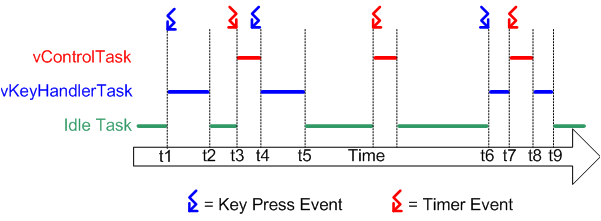
\includegraphics[width=0.8\textwidth]{figures/FreeRTOS_Prioritization.png}
  \caption{Scheduling of three tasks with prioritization~\cite{SchedulingRTOS}.}
  \label{fig:freertosprio}
\end{figure}


Because the scheduler is much more complex, prioritization is also possible in \gls{frtos}. Figure~\ref{fig:freertosprio} illustrates how the scheulder can be instructed to prioritize certain tasks, in this case vControlTask, higher than vKeyHandlerTask, which is again prioritised higher than the idle task. This concept is not supported in Protothreads, and can only be simulated partially by scheduling a task more frequently than another, which has drawbacks as well.


\subsection{Summary}\label{subsec:concurrencysummary}
\gls{frtos} is more powerful than Protothreads, with a powerful scheduler supporting multiple concurrency models. However, compared to Protothreads it also has a much larger memory footprint, especially as the amount of tasks in the program increases.

To focus on the design of a programming language aimed at hobbyists - with few surprises, such as surprising memory constraints - the simpler Protothreads library is chosen for this project. This limits the options available for language constructs related to concurrency in the design of the programming language, but should still be enough for a small language.